\documentclass[letterpaper,12pt]{article}
\usepackage{tabularx} % extra features for tabular environment
\usepackage{amsmath}  % improve math presentation
\usepackage{float}
\usepackage{pdfpages}

\usepackage{graphicx} % takes care of graphic including machinery
\graphicspath{ {./figures/} }
\usepackage[margin=1in,letterpaper]{geometry} % decreases margins
\usepackage{cite} % takes care of citations
\usepackage[final]{hyperref} % adds hyper links inside the generated pdf file
\hypersetup{
	colorlinks=true,       % false: boxed links; true: colored links
	linkcolor=blue,        % color of internal links
	citecolor=blue,        % color of links to bibliography
	filecolor=magenta,     % color of file links
	urlcolor =blue         
}




\begin{document}

\title{Spring 2022 EE214 Experiment 1  \protect\\ Diodes and Rectifiers}
\author{Ahmet Akman 2442366 \protect\\ Yusuf Toprak Yıldıran 2444149}
\date{\today}
\maketitle
\tableofcontents
%\begin{abstract}
%abstract
%\end{abstract}
\section{Introduction}
In this experiment ,  characteristics of different  diodes ,and rectifiers are investigated. First the i-v characteristics of 3 different diodes are expected to be oobserved. Then, the behavior of the half wave is expected to be experimented. Lastly, observations are made on clamper and  zener regulator circuits. The results of the experimentation is presented in this document.
\section{Experimental Results and Discussion}
The results of the experiment are discussed in following steps.
\subsection{Step 1}
In this step, the circuit schematic given in Figure TODO is constructed on breadboard. As the signal supply, analog signal generator is used for floating output.
\begin{figure}[H]
\centering
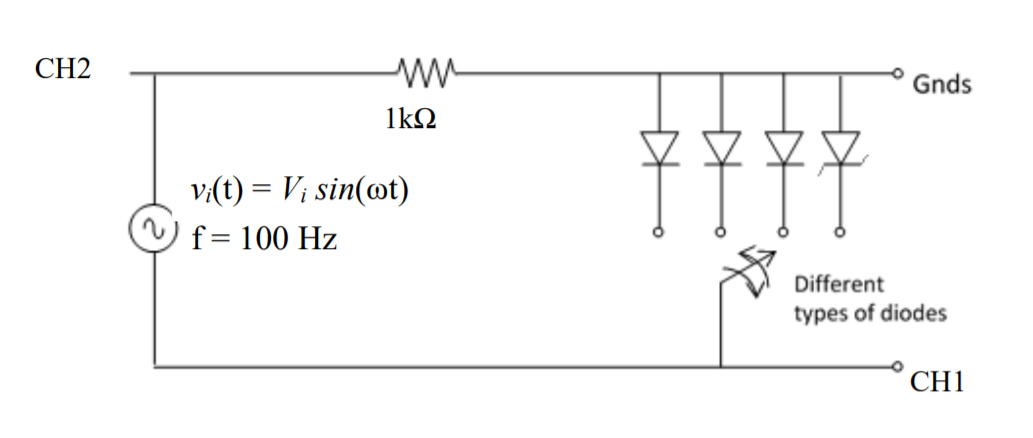
\includegraphics[width=1\textwidth]{1_1.png}
\caption{Circuit schematic for the step 1}
\end{figure} 

\subsubsection{a)}
%\href{https://www.vishay.com/docs/88503/1n4001.pdf}{1N40007} 
The diode models, \href{https://logosfoundation.org/elektron/mixers/AA119.pdf}{AA119},href{https://www.vishay.com/docs/88536/ba157.pdf}{BA159}  ,and \href{https://www.vishay.com/docs/85604/bzx55.pdf}{BZX55C-6V2} are used. The probes of the oscilloscope is connected to the nodes indicated in Figure TODO. The resulting graph is plotted as given in Figure TODO2 TODO3 ,and TODO 4 for 
\href{https://logosfoundation.org/elektron/mixers/AA119.pdf}{AA119},href{https://www.vishay.com/docs/88536/ba157.pdf}{BA159}  ,and \href{https://www.vishay.com/docs/85604/bzx55.pdf}{BZX55C-6V2} respectively.
Using those plots the piecewise parameters of the diodes are obtained by the virtue of the cursors of the oscilloscope. The parameters of diode AA119 is given in Table 1.

\begin{table}[H]
    \centering
    \caption{Piecewise parameters of diode AA119}
    \begin{tabular}{||c | c | c||}
    \(V_{on}\) & 350 mV \\
    \(r_f\) & 0.17 \(\Omega\) \\
    \(r_r\) & 86 \(\Omega\)
    \end{tabular}
\end{table}
The obtained parameters of diode AA119 is given in Table 2.
\begin{table}[H]
    \centering
    \caption{Piecewise parameters of diode BA159}
    \begin{tabular}{||c | c | c||}
    \(V_{on}\) & 973.5 mV \\
    \(r_f\) & 0.625 \(\Omega\) \\
    \(r_r\) & 86.2 \(\Omega\)
    \end{tabular}
\end{table}
The obtained parameters of diode BZX55C-6V2 is given in Table 3.
\begin{table}[H]
    \centering
    \caption{Piecewise parameters of diode BZX55C-6V2}
    \begin{tabular}{||c | c | c||}
    \(V_{on}\) & 752 mV \\
    \(V_{z}\) & 5.92V \\
    \(r_f\) & 0.05 \(\Omega\) \\
    \(r_r\) & 0.156 \(\Omega\)
    \end{tabular}
\end{table}
So, the pimple i-v characteristics of 3 different diodes are obtained ,and analyzed using the plot.

\subsubsection{b)}

\subsection{Step 2}

\begin{figure}[H]
    \centering
    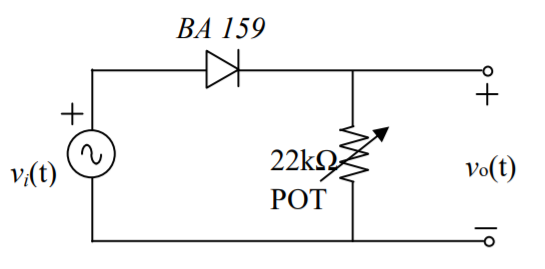
\includegraphics[width=1\textwidth]{2_1.png}
    \caption{Circuit schematic for the step 2}
\end{figure} 
    
\subsubsection{a)}
\subsubsection{b)}


\subsection{Step 3}

\begin{figure}[H]
    \centering
    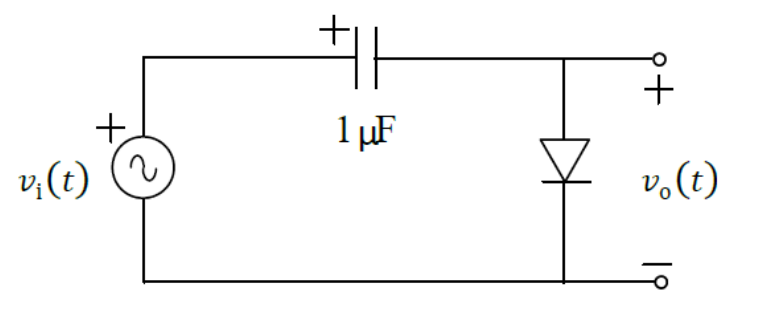
\includegraphics[width=1\textwidth]{3_1.png}
    \caption{Circuit schematic for the step 3}
\end{figure} 
    
    

\subsection{Step 4}

\begin{figure}[H]
    \centering
    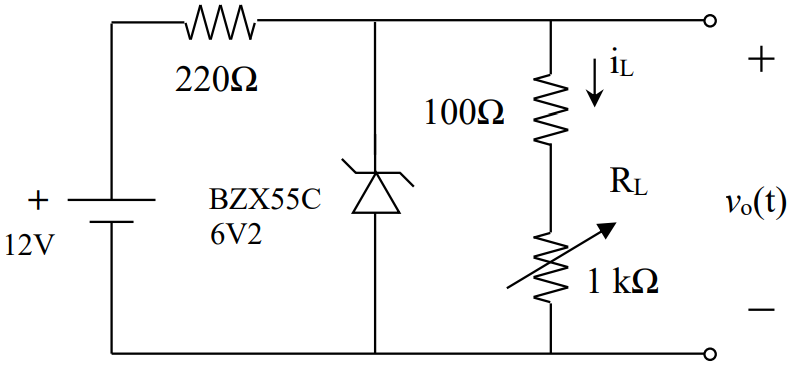
\includegraphics[width=1\textwidth]{4_1.png}
    \caption{Circuit schematic for the step 4}
\end{figure} 
    
    
\section{Conclusion}
asdfd
\section*{Appendix A}
\begin{itemize}
    \item PreLab Preprataion 6 hours
    \item Experimental Work 2  hours
    \item Report Wrining 6 hours
\end{itemize}

\end{document}

%%%%%%%%%%%%%%%%%%%%%%   EXAMPLE TABLE   %%%%%%%%%%%%%%%%%%%%%%%%%%%%%%%%
\begin{table}[H]
\begin{center}
    \caption{Resistance reading by color code convention.}
    \vspace{2mm}
    \begin{tabular}{||c | c | c||} 
        \hline
        Color Order & Value & Tolerance \\ [0.5ex] 
        \hline\hline
        Brown / Black / Red / Gold & 1k\( \Omega \) & \( \% \) 5  \\ 
        \hline
        Yellow / Violet / Red / Gold & 4.7k\( \Omega \) & \( \% \) 5   \\
        \hline
        Brown / Grey / Orange / Gold & 18k\( \Omega \) & \( \% \) 5  \\ [1ex] 
        \hline
    \end{tabular}
\end{center}
\end{table}


%%%%%%%%%%%%%%%%%%%%%%   EXAMPLE IMAGE   %%%%%%%%%%%%%%%%%%%%%%%%%%%%%%%%
\begin{figure}[H]
\centering
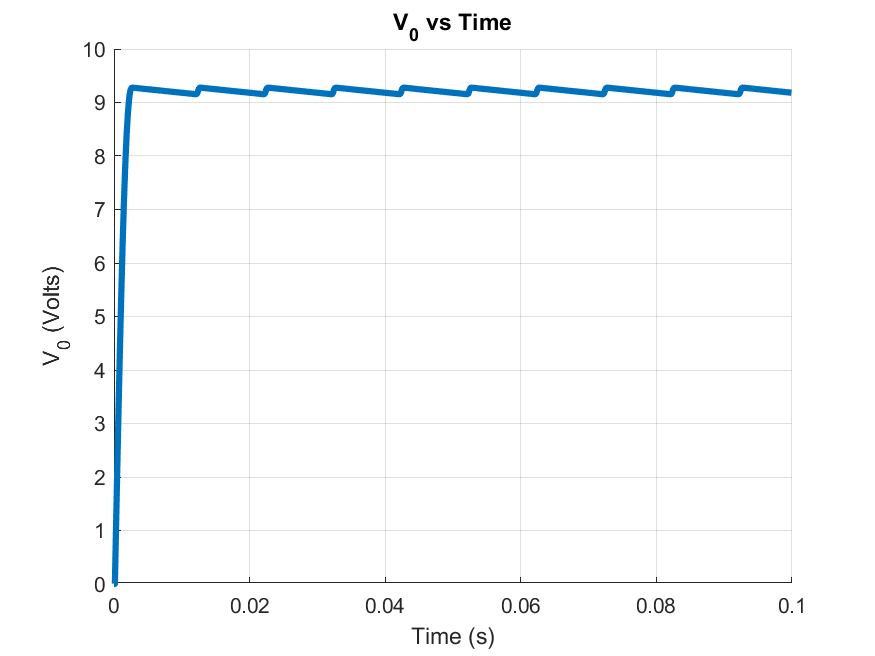
\includegraphics[width=1\textwidth]{5.png}
\caption{Circuit schematic for the step 5}
\end{figure} 

%%%%%%%%%%%%%%%%%%%%%%   EXAMPLE IMAGE FROM PDF   %%%%%%%%%%%%%%%%%%%%%%%%%%%%%%%%
\begin{figure}[H] \centering{
	\includegraphics[scale=0.25]{2a_plot.pdf}}
	\caption{Experiment 2}
\end{figure}
	